\documentclass[twocolumn, 12pt]{article}    % two-column because cheat sheets fit like that
\usepackage[utf8]{inputenc}
\usepackage{amsmath}    % allows math to happen
\usepackage{marvosym}
\usepackage{textcomp}
\usepackage{geometry}   % allows you to change the margins and headers/footers, and more
\usepackage{array}
\usepackage{wrapfig}
\usepackage{multirow} 
\usepackage{graphicx}   % allows for inclusion of graphics or several types, i think
\usepackage{float}      % SUPER  IMPORTANT. lets you tell LaTeX where to put your graphics, as opposed to where it feels
\usepackage{wrapfig}    % Lets text wrap around figures, more relevant for reports really
\usepackage{caption}
\usepackage{amssymb}    
\usepackage{ulem}       % allows strikethrough and some
\usepackage[table]{xcolor}  % enhances tables by allowing colors to happen. notably, as background/fill colors
\usepackage{bondgraph}  % allows bond graphs
\usepackage{caption}    % lots of control of captions and caption geometries
\usepackage{ragged2e}
\geometry{margin=.5in}      % this allows for a lot to fit on the page
\usepackage{wrapfig} % for text wrapping around images
\usepackage{multicol} % allows for multi column enviornment


\begin{document}
\footnotesize
\RaggedRight
%%
\section*{Mechanics of Materials}

\begin{equation*}
     \sigma_N=\frac{ P}{A} \hspace{30pt} \sigma_B = -\frac{My}{I}\hspace{30pt} \tau =\frac{Tr}{I_p}
\end{equation*}
\begin{equation*}
    \tau_s = \frac{V}{A} \hspace{30pt} \tau_T = \frac{VQ}{Ib} \hspace{30pt} \Bar{y} = \frac{\Sigma ydA }{\Sigma dA}
\end{equation*}
\begin{equation*}
    \varepsilon_0=\frac{\Delta L}{L_0} \hspace{5pt} \text{(nominal)} \hspace{30pt} \varepsilon = \int_{L_0}^L \frac{dL}{L} = ln(1-\varepsilon_0) \hspace{5pt} \text{(true)}
\end{equation*}
\begin{equation*}
    \sigma = \frac{P}{A} \hspace{5pt} \text{(nominal)} \hspace{30pt} \sigma = \sigma_0(1+\varepsilon_0) \hspace{5pt} \text{(true)}
\end{equation*}
\begin{equation*}
    \text{thin-wall} \hspace{30pt}\sigma_H(\text{hoop})=\frac{pr}{t} \hspace{30pt} \sigma_L(\text{axial})=\frac{pr}{2t}
\end{equation*}
\subsubsection*{For equilibrium}
\begin{align*}
    0 &=  \frac{\partial{\tau_{xx}}}{\partial{x}} +  \frac{\partial{
    \tau_{xy}}}{\partial{y}} +  \frac{\partial{\tau_{xz}}}{\partial{z}} + F_z\\
    0 &=  \frac{\partial{\tau_{yx}}}{\partial{x}} +  \frac{\partial{
    \tau_{yy}}}{\partial{y}} +  \frac{\partial{\tau_{yz}}}{\partial{z}} + F_y\\
    0 &=  \frac{\partial{\tau_{zx}}}{\partial{x}} +  \frac{\partial{
    \tau_{zy}}}{\partial{y}} +  \frac{\partial{\tau_{zz}}}{\partial{z}} + F_z\\
\end{align*}
\begin{center}
    (Typically, \(F_x=F_y=F_z=0\))
\end{center}
%%
\subsubsection*{Plane Stress}
\begin{equation*}
    \sigma_{x'} =\frac{1}{2}(\sigma_x+\sigma_y) + \frac{1}{2}(\sigma_x-\sigma_y) cos2\theta +\tau_{xy}sin2\theta
\end{equation*}
\begin{equation*}
    \sigma_{y'} =\frac{1}{2}(\sigma_x+\sigma_y) - \frac{1}{2}(\sigma_x-\sigma_y) cos2\theta -\tau_{xy}sin2\theta
\end{equation*}
\begin{equation*}
    \tau_{x'y'} =-\frac{1}{2}(\sigma_x-\sigma_y) sin2\theta +\tau_{xy}cos2\theta
\end{equation*}
\begin{equation*}
    \sigma_{x'}+\sigma_{y'}=\sigma_x+\sigma_y \hspace{30pt} tan(2\theta_p)= \frac{2\tau_{xy}}{\sigma_x-\sigma_y}
\end{equation*}
\begin{equation*}
    \sigma_{1,2} =\frac{\sigma_x+\sigma_y}{2} \pm \sqrt{\left(\frac{\sigma_x-\sigma_y}{2}\right)^2 +\tau_{xy}^2} 
\end{equation*}
%%
\subsubsection*{3D Stress}
\begin{equation*}
    det(\tau -\lambda I) = 0 \hspace{10pt}\Longrightarrow \hspace{10pt}\lambda = \sigma_1,\sigma_2,\sigma_3
\end{equation*}
\begin{itemize}
    \item Can use Mohr's circle \emph{only} if 4+ shear stresses = 0\\
    \item Each circle on Mohr's circle is drawn as if looking down each principal direction axis at the element in principal stresses. 
\end{itemize}
\begin{equation*}
    M= \begin{bmatrix}
    x'\cdot x & x'\cdot y & x' \cdot z\\
    y'\cdot x & y'\cdot y & y' \cdot z\\
    z'\cdot x & z'\cdot y & z' \cdot z\\
\end{bmatrix} = 
\begin{bmatrix}
    \begin{bmatrix}
        & \text{eigenvector 1} &\\
    \end{bmatrix}\\
    \begin{bmatrix}
        & \text{eigenvector 2} &\\
    \end{bmatrix}\\
    \begin{bmatrix}
        & \text{eigenvector 3} &\\
    \end{bmatrix}
\end{bmatrix}
\end{equation*}
\begin{center}
    The eigenvectors describe directions of the principal stresses 
\end{center}
\begin{equation*}
    \tau' = M\tau M^T
\end{equation*}
\begin{equation*}
    t=\tau n = \sigma + \tau(\text{single shear}) \hspace{30pt} t=\tau n = \lambda n  
\end{equation*}
\begin{equation*}
    t -(t\cdot n)n = \tau
\end{equation*}
%% 
\subsubsection*{Strain}
Superposition of \(u,v,w\) is valid if linearly elastic or small displacements 
\begin{equation*}
    \varepsilon_x =  \frac{\partial{u}}{\partial{x}} \hspace{30pt} 
    \gamma_{xy}=\gamma_{yx} =  \frac{\partial{u}}{\partial{y}} +  \frac{\partial{v}}{\partial{x}} 
\end{equation*}
\begin{equation*}
    \varepsilon_y = \frac{\partial{v}}{\partial{y}} \hspace{30pt} \gamma_{yz}=\gamma_{zy} = \frac{\partial{v}}{\partial{z}} +  \frac{\partial{w}}{\partial{y}}
\end{equation*}
\begin{equation*}
    \varepsilon_z =  \frac{\partial{w}}{\partial{z}} \hspace{30pt}  \gamma_{xz}=\gamma_{zx} =  \frac{\partial{w}}{\partial{x}} + \frac{\partial{u}}{\partial{z}}
\end{equation*}
\begin{equation*}
    \varepsilon = \begin{bmatrix}
        \varepsilon_x & \frac{1}{2}\gamma_{xy} & \frac{1}{2}\gamma_{xz}\\
        \frac{1}{2}\gamma_{yx} & \varepsilon_y & \frac{1}{2}\gamma_{yz}\\
        \frac{1}{2}\gamma_{zx} & \frac{1}{2}\gamma_{zy} & \varepsilon_z\\
    \end{bmatrix}
\end{equation*}
\begin{equation*}
    \varepsilon' = M\varepsilon M^T
\end{equation*}
\begin{equation*}
    e = \frac{\Delta V}{V_0} = \varepsilon_x + \varepsilon_y+
    \varepsilon_z = \text{dilitation}
\end{equation*}
Mohr's circle can be used \emph{only} with tensorial strains


%%
\underline{Strain Compatibility}\\
Satisfy \emph{all} to ensure compatibility
\begin{equation*}
     \frac{\partial^2{\varepsilon_x}}{\partial{y^2}} +  \frac{\partial^2{
     \varepsilon_y}}{\partial{x^2}} =  \frac{\partial^2{\gamma_{xy}
     }}{\partial x\partial y}      \hspace{30pt}  \frac{\partial^2{\varepsilon_y}}{\partial{z^2}} +  \frac{\partial^2{
     \varepsilon_z}}{\partial{y^2}} =  \frac{\partial^2{\gamma_{yz}
     }}{\partial y\partial z}     
\end{equation*}
\begin{equation*}
    \frac{\partial^2{\varepsilon_z}}{\partial{x^2}} +  \frac{\partial^2{
     \varepsilon_x}}{\partial{z^2}} =  \frac{\partial^2{\gamma_{xz}
     }}{\partial x\partial z} 
\end{equation*}
\begin{equation*}
    2 \frac{\partial^2{\varepsilon_x}}{\partial y \partial z} =  \frac{\partial{}}{\partial{x}} \left( - \frac{\partial{\gamma_{yz}}}{\partial{x}} +  \frac{\partial{\gamma_{xz}}}{\partial{y}}  +  \frac{\partial{
     \gamma_{xy}}}{\partial{z}} \right)
\end{equation*}
\begin{equation*}
    2 \frac{\partial^2{\varepsilon_y}}{\partial x \partial z} =  \frac{\partial{}}{\partial{y}} \left( \frac{\partial{\gamma_{yz}}}{\partial{x}} -  \frac{\partial{\gamma_{xz}}}{\partial{y}}  +  \frac{\partial{
     \gamma_{xy}}}{\partial{z}} \right)
\end{equation*}
\begin{equation*}
    2 \frac{\partial^2{\varepsilon_z}}{\partial x \partial y} =  \frac{\partial{}}{\partial{z}} \left( \frac{\partial{\gamma_{yz}}}{\partial{x}} +  \frac{\partial{\gamma_{xz}}}{\partial{y}}  -  \frac{\partial{
     \gamma_{xy}}}{\partial{z}} \right)
\end{equation*}


%%
\subsubsection*{Hooke's Law}
\begin{equation*}
    \sigma = \sigma(\varepsilon)=\tau(\varepsilon) \hspace{30pt}  \tau =c\varepsilon \hspace{5pt} \text{(or)} \hspace{5pt} \varepsilon=c^{-1}\tau
\end{equation*}
\underline{Uniaxial}\\
\begin{equation*}
     \sigma = E\varepsilon \hspace{30pt }\nu=-\frac{\text{lateral strain}}{\text{axial strain}} \hspace{30pt} \varepsilon_y=\varepsilon_z = -\nu \frac{\sigma_x}{E}
\end{equation*}

\underline{Isotropic}\\
\begin{equation*}
    G = \frac{E}{2(1+\nu)}
\end{equation*}
\begin{equation*}
    \begin{bmatrix}
        \varepsilon_{xx} \\
        \varepsilon_{yy}\\
        \varepsilon_{zz}\\
        \varepsilon_{yz}\\
        \varepsilon_{zx}\\
        \varepsilon_{xy}
    \end{bmatrix}
    =\frac{1}{E}
    \begin{bmatrix}
        1 & -\nu & -\nu & 0 &0 &0\\
        -\nu &1 & -\nu &0 &0 &0\\
        -\nu &-\nu &1 &0 &0 &0\\
        0 & 0 & 0 & 1+\nu & 0 &0\\
        0 & 0 & 0 & 0 & 1+\nu & 0\\
        0 & 0 & 0 & 0 &0 & 1+\nu
    \end{bmatrix}
    \begin{bmatrix}
        \tau_{xx}\\
        \tau_{yy}\\
        \tau_{zz}\\
        \tau_{yz}\\
        \tau_{zx}\\
        \tau_{xy}
    \end{bmatrix}
\end{equation*}
\begin{equation*}
    \begin{bmatrix}
        \tau_{xx}\\
        \tau_{yy}\\
        \tau_{zz}\\
        \tau_{yz}\\
        \tau_{zx}\\
        \tau_{xy}
    \end{bmatrix} =
    \begin{bmatrix}
        2\mu+\lambda & \lambda & \lambda & 0 &0 &0\\
        \lambda &2\mu+\lambda & \lambda &0 &0 &0\\
        \lambda & \lambda &2\mu+\lambda &0 &0 &0\\
        0 & 0 & 0 & \mu & 0 &0\\
        0 & 0 & 0 & 0 & \mu & 0\\
        0 & 0 & 0 & 0 &0 & \mu
    \end{bmatrix}
    \begin{bmatrix}
        \varepsilon_{xx} \\
        \varepsilon_{yy}\\
        \varepsilon_{zz}\\
        2\varepsilon_{yz}\\
        2\varepsilon_{zx}\\
        2\varepsilon_{xy}
    \end{bmatrix}
\end{equation*}
\begin{equation*}
    \text{where     } \lambda =\frac{\nu E}{(1+\nu)(1-2\nu)} \text{     and     } \mu = G
\end{equation*}
\begin{equation*}
    \text{Bulk elasticity }K = \frac{E}{3(1-2\nu)} \text{ (hydrostatic cond.)}
\end{equation*}


\underline{Transverse Isotropy}\\
Behavior is identical in directions 2 and 3, not 1
\begin{equation*}
    \frac{1}{G_{23}} = \frac{2(1+\nu_{23})}{E_2} \hspace{20pt} E_2=E_3 \hspace{20pt} \nu_{12} =\nu_{13} \hspace{20pt}G_{12}=G_{13}
\end{equation*}
\begin{equation*}
    \begin{bmatrix}
        \varepsilon_{xx} \\
        \varepsilon_{yy}\\
        \varepsilon_{zz}\\
        \varepsilon_{yz}\\
        \varepsilon_{zx}\\
        \varepsilon_{xy}
    \end{bmatrix} = 
    \begin{bmatrix}
        \frac{1}{E_1} & -\frac{\nu_{12}}{E_1} & -\frac{\nu_{12}}{E_1} &0 &0 &0\\
        \frac{-\nu_{12}}{E_1} & \frac{1}{E_2} & -\frac{\nu_{23}}{E_2} &0 &0 &0\\
        -\frac{\nu_{12}}{E_1} & -\frac{\nu_{23}}{E_2} & \frac{1}{E_2} &0 &0 &0\\
        0& 0 &0 &\frac{1}{G_{12}} &0 &0\\
        0& 0 &0 &0 &\frac{1}{G_{23}} &0 \\
        0 &0 &0 &0 &0 &\frac{1}{G_{12}}\\
    \end{bmatrix}
    \begin{bmatrix}
        \tau_{xx}\\
        \tau_{yy}\\
        \tau_{zz}\\
        \tau_{yz}\\
        \tau_{zx}\\
        \tau_{xy}
    \end{bmatrix}
\end{equation*}

\underline{Orthotropic}\\
Behavior is different in each principal direction
\begin{equation*}
        \begin{bmatrix}
        \varepsilon_{xx} \\
        \varepsilon_{yy}\\
        \varepsilon_{zz}\\
        \varepsilon_{yz}\\
        \varepsilon_{zx}\\
        \varepsilon_{xy}
    \end{bmatrix} = 
    \begin{bmatrix}
        \frac{1}{E_1} & -\frac{\nu_{21}}{E_2} & -\frac{\nu_{31}}{E_3} &0 &0 &0\\
        \frac{-\nu_{12}}{E_1} & \frac{1}{E_2} & -\frac{\nu_{32}}{E_3} &0 &0 &0\\
        -\frac{\nu_{13}}{E_1} & -\frac{\nu_{23}}{E_2} & \frac{1}{E_3} &0 &0 &0\\
        0& 0 &0 &\frac{1}{G_{12}} &0 &0\\
        0& 0 &0 &0 &\frac{1}{G_{23}} &0 \\
        0 &0 &0 &0 &0 &\frac{1}{G_{13}}\\
    \end{bmatrix}
    \begin{bmatrix}
        \tau_{xx}\\
        \tau_{yy}\\
        \tau_{zz}\\
        \tau_{yz}\\
        \tau_{zx}\\
        \tau_{xy}
    \end{bmatrix}
\end{equation*}
\begin{equation*}
    \text{Maxwell's recip:} \hspace{10pt} \frac{\nu_{12}}{E_1} = \frac{\nu_{21}}{E_2} \hspace{20pt} \frac{\nu_{13}}{E_1}=\frac{\nu_{31}}{E_3} \hspace{20pt} \frac{\nu_{23}}{E_2}=\frac{\nu_{32}}{E_3}
\end{equation*}

\subsubsection*{Strain Energy}
\begin{equation*}
    U_0 = \frac{1}{2}(\sigma_x\varepsilon_x +\sigma_y\varepsilon_y + \sigma_z\varepsilon_z + \tau_{xy}\gamma_{xy} + \tau_{yz}\gamma_{yZ} + \tau_{xz}\gamma_{xz})
\end{equation*}


\subsubsection*{Failure Theories}
\underline{Ductile}
\begin{itemize}
    \item Max Normal: \hspace{75pt} \(|\sigma_1,\sigma_2,\sigma_3| \geq \sigma_y, \sigma_u\)
    \item Max Shear Stress/Tresca: \hspace{10pt} \(\tau_{max}=(\sigma_1- \sigma_3) \geq \sigma_y\)
    \item Von Mises/Distortional Energy:\\
        \begin{align*}
            2\sigma_{yp}^2 =&  (\sigma_x-\sigma_y)^2 + (\sigma_y- \sigma_z)^2 + (\sigma_z-\sigma_x)^2\\
             & + 6(\tau_{xy}^2 +\tau_{yz}^2 + \tau_{xz}^2) 
        \end{align*}
    
        OR \hspace{3.5pt} \(2\sigma_{yp}^2 = (\sigma_1 - \sigma_2)^2 + (\sigma_2 - \sigma_3)^2 - (\sigma_3 - \sigma_1)^2\)
    \item Octahedral Shear: \hspace{70pt} \(\tau_{oct} = 0.47 \sigma_{yp}\)
    \item Tresca is more conservative, VM is more accurate
    \item Bigger parts are more conservative
\end{itemize}
\underline{Brittle}\\
\(\sigma_u\) for tensile, \(\sigma_{u'}\) for compressive\\
\begin{itemize}
    \item Max Normal: same as ductile, but allows \(\sigma_u \neq \sigma_{u'}\) 
    \item Coulomb-Mohr: \hspace{50pt}  \(\sigma_1/\sigma_u - \sigma_3/\sigma_{u'} = 1/n\)
    \item Coulomb-Mohr is conservative, max normal is liberal
\end{itemize}

\subsubsection*{Cracks}
\begin{equation*}
    K = \lambda \sigma_{nom}\sqrt{\pi a} \hspace{20pt} [MPa \cdot m^{1/2}] \hspace{20pt} \text{valid if} \hspace{5pt} a,t \geq K_c^2/\sigma_{yp}^2
\end{equation*}
\begin{figure}[h!]
    \centering
    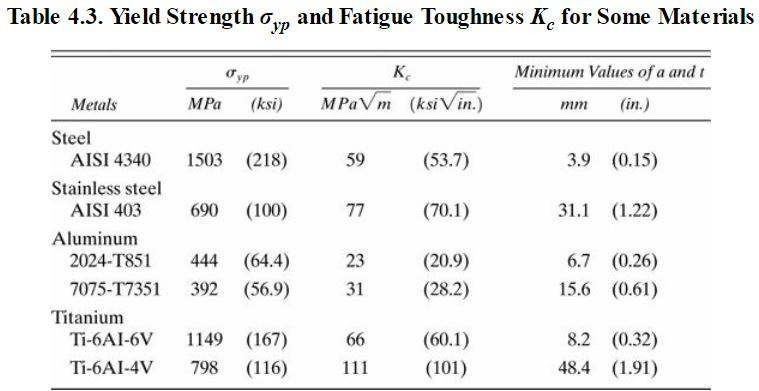
\includegraphics[width=0.4\textwidth]{FatigueCrackToughnessFactors.jpg}
\end{figure}

\subsubsection*{Fatigue}
\begin{equation*}
    N_{CR} = N_f\left(\frac{\sigma_{CR}}{\sigma_f} \right)^{1/b} \hspace{17.5pt} b = \frac{ln(\sigma_f/ \sigma_e)}{ln(N_f / N_e )} \hspace{17.5pt} \sigma_e < \sigma_{CR} < \sigma_f
\end{equation*}
\begin{equation*}
    \sigma_m = \frac{1}{2}(\sigma_{max} + \sigma_{min}) \hspace{30pt} \sigma_a = 
    \frac{1}{2}(\sigma_{max} - \sigma_{min})
\end{equation*}
\underline{Fatigue Criteria}\\
\begin{itemize}
    \item Modified Goodman: \hspace{20pt} \(\sigma_a / \sigma_{CR} + \sigma_m / \sigma_u = 1/n\)
    \item Soderberg: \hspace{57.5pt} \(\sigma_a / \sigma_{CR} + \sigma_m / \sigma_{yp} = 1/n\)
    \item Gerber: \hspace{62.5pt} \(\sigma_a / \sigma_{CR} + (\sigma_m / \sigma_u)^2 = 1/n \)
    \item SAE: \hspace{87.5pt} \( \sigma_a /\sigma_{CR} + \sigma_m / \sigma_f = 1/n \)
\end{itemize}
\begin{figure}[h!]
    \centering
    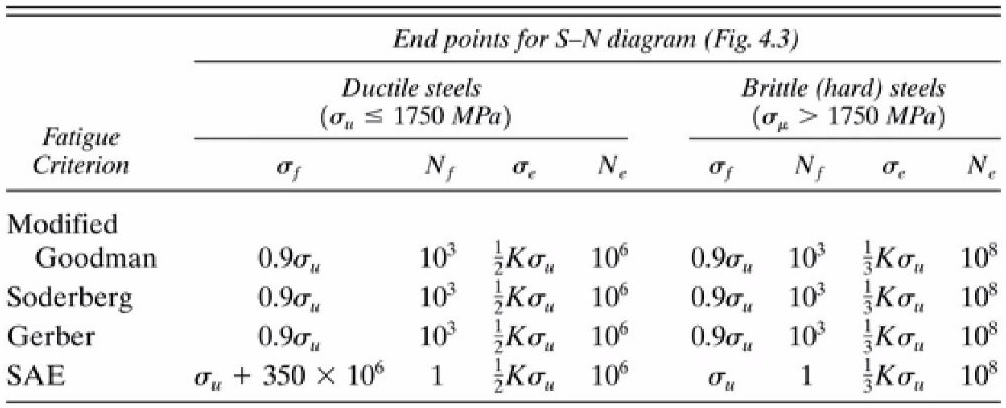
\includegraphics[width=0.4\textwidth]{FatigueTable.jpg}
\end{figure}


\subsubsection*{Dynamic Loading}
\begin{equation*}
    \text{Vertical:} \hspace{12.5pt} \delta_{max} = \delta_{st} \left(1+\sqrt{1+ \frac{2h}{\delta_{st}}} \right) = \kappa\delta_{st} \hspace{12.5pt} P_{dyn} = \kappa W
\end{equation*}
\begin{equation*}
    \text{Horizontal:} \hspace{30pt} \delta_{max} = \delta_{st}\sqrt{\frac{v^2}{g\delta_{st}}} \hspace{30pt} P_{dyn} = W \sqrt{\frac{v^2}{d\delta_{st}}}
\end{equation*}

\subsubsection*{Theory of Elasticity}
Typically, body forces equal zero.\\
\underline{Plane Strain}\\
\begin{equation*}
    \left(  \frac{\partial{^2}}{\partial{x^2}} +  \frac{\partial{^2}}{\partial{y^2}} \right)(\sigma_x + \sigma_y) = -\frac{1}{1-\nu} \left( \frac{\partial{F_x}}{\partial{x}} + \frac{\partial{F_y}}{\partial{y}} \right)
\end{equation*}
\underline{Plane Stress}\\
\begin{equation*}
    \left(  \frac{\partial{^2}}{\partial{x^2}} +  \frac{\partial{^2}}{\partial{y^2}} \right)(\sigma_x + \sigma_y) = -(1+\nu) \left( \frac{\partial{F_x}}{\partial{x}} + \frac{\partial{F_y}}{\partial{y}} \right)
\end{equation*}
\underline{Airy's Stress Function}\\
\begin{equation*}
    \text{Define } \Phi(x,y) \longrightarrow \sigma_x = \frac{\partial{^2 \Phi}}{\partial{y^2}}   \hspace{15pt} \sigma_y =  \frac{\partial{^2 \Phi}}{\partial{x^2}} \hspace{15pt} \tau_{xy} = - \frac{\partial{^2 \Phi}}{\partial x \partial y} 
\end{equation*}
\noindent to satisfy and boundary conditions, and
\begin{equation*}
     \frac{\partial{^4 \Phi}}{\partial{x^4}} + 2  \frac{\partial{^4 \Phi}}{\partial{x^2} \partial y^2} +  \frac{\partial{^4 \Phi}}{\partial{y^4}} = \nabla ^4\Phi = 0
\end{equation*}


\subsubsection*{Concentrated Loads}

\begin{figure}[h!]
    \centering
    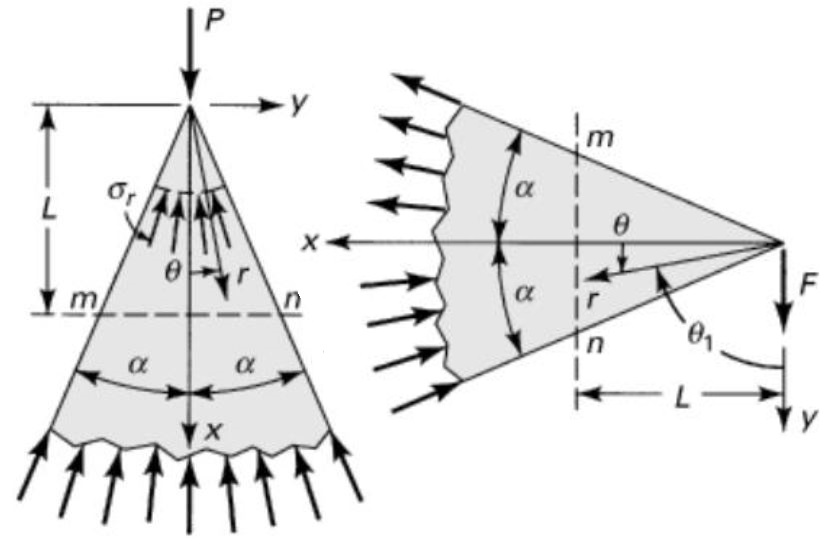
\includegraphics[width=0.33\textwidth]{SemiInfiniteWedges.jpg}
\end{figure}
\begin{multicols}{2}
\begin{center}
    \underline{Normal}
\end{center}
\begin{equation*}
    \sigma_r = -\frac{Pcos(\theta)}{r(\alpha + \frac{1}{2}sin\alpha)}
\end{equation*}
\begin{equation*}
    \sigma_\theta = \tau_{r\theta} = 0
\end{equation*}
\begin{align*}
    \sigma_x =& \sigma_r cos^2(\theta)\\ 
    =& \frac{-Pcos^4(\theta)}{L(\alpha +\frac{1}{2}sin(2\alpha)}\\
\end{align*}
\begin{equation*}
        \sigma_y = \tau_{xy} = 0
\end{equation*}
\vspace{5pt}


\begin{center}
    \underline{Bending}
\end{center}
\begin{equation*}
    \sigma_r = -\frac{Fcos(\theta)}{r(\alpha - \frac{1}{2}sin\alpha)}
\end{equation*}
\begin{equation*}
    \sigma_\theta = \tau_{r\theta} = 0
\end{equation*}
\begin{align*}
    \sigma_x =& \frac{-F}{\alpha -\frac{1}{2} sin(2\alpha)} \frac{x^2y}{(x^2 + y^2)^2}\\
    \sigma_y =& \frac{-F}{\alpha -\frac{1}{2} sin(2\alpha)} \frac{y^3}{(x^2 + y^2)^2}\\
    \tau_{xy} =& \frac{-F}{\alpha -\frac{1}{2} sin(2\alpha)} \frac{xy^2}{(x^2 + y^2)^2}\\
\end{align*}
\end{multicols}

Semi-infinite plate (\(\alpha = \pi/2\)):\\
\begin{equation*}
    \sigma_r = -\frac{2P}{\pi} \frac{cos(\theta)}{r} \hspace{30pt} \sigma_\theta = \tau_{r\theta} = 0
\end{equation*}


\subsubsection*{Stress Concentrations}
\begin{equation*}
    K =\frac{\text{max stress}}{\text{nominal stress}} = \frac{\sigma_{max}}{\sigma_{nom}} \hspace{30pt} \text{//tabulated}
\end{equation*}
\underline{Uni-axial Tension (hole)}\\
\begin{equation*}
    \sigma_r = \frac{1}{2}\sigma_0 \left[ \left( 1 -\frac{a^2}{r^2} \right) + \left(1 + \frac{3a^4}{r^4} -\frac{4a^2}{r^2} \right) cos(2\theta)\right]
\end{equation*}
\begin{equation*}
    \sigma_\theta = \frac{1}{2}\sigma_0 \left[ \left( 1 +\frac{a^2}{r^2} \right) - \left(1 + \frac{3a^4}{r^4} \right) cos(2\theta)\right]
\end{equation*}
\begin{equation*}
    \tau_{r\theta} = -\frac{1}{2}\sigma_0 \left(1 - \frac{3a^4}{r^4} + \frac{4a^2}{r^2} \right) cos(2\theta)
\end{equation*}
Theory of elasticity allows for superposition if bi/tri-axial. 
\begin{equation*}
    \text{Elliptical hole:} \hspace{20pt} K = 1+ 2(b/a) \hspace{20pt}  \sigma_{max} = K \sigma_0 \hspace{20pt} 2b>2a
\end{equation*}




\subsubsection*{Contact Stresses}
\underline{Spheres} \hspace{125pt} \(P_0 = (1.5F)/(\pi a^2)\)\\
\begin{equation*}
    a = \left(\frac{3F}{4} \frac{(1-\nu_1^2)/E_1 + (1-\nu_2^2)/E_2 }{1/r_1 + 1/r_2} \right)^{1/3} \hspace{20pt} area = \pi a^2
\end{equation*}
\begin{equation*}
    a = 0.88 \left( \frac{F(E_1+E_2)r_1r_2}{ E_1E_2(r_1+ r_2)} \right)^{1/3} \hspace{30pt} \text{if} \hspace{10pt} \nu_1=\nu_2 \approx 0.3
\end{equation*}
\begin{equation*}
    \hspace{-15pt} \delta^* = 0.77 \left[ F^2 \left(\frac{1}{E_1} + \frac{1}{E_2} \right)^2 \left(\frac{1}{r_1} + \frac{1}{r_2} \right) \right]^{1/3}  \text{if} \hspace{5pt} \nu_1=\nu_2 \approx 0.3
\end{equation*}
\begin{center}
    \(^*\) relative displacement of sphere centers\\
\end{center}
\vspace{-10pt}
Flat surface, \(r_2 \rightarrow \infty\). Spherical cup, \( r_2 \rightarrow -r_2 \)\\
\textit{Induced Stresses at Contact}\\
Loading in \(z\) direction, \(z\) is distance from contact surface
\begin{equation*}
    \hspace{-30pt} \sigma_x(z) = \sigma_y(z) = -P_0 \left[ \left( 1 - \frac{z}{a} atan\left(  \frac{1}{z/a}\right) \right) (1+\nu) - \frac{1}{2[1 + (z/a)^2]} \right]
\end{equation*}
\begin{equation*}
    \sigma_z(z) = \frac{-P_0}{1+(z/a)^2} \hspace{20pt} \tau_{yz} = \tau_{xz} = \frac{1}{2}(\sigma_x - \sigma_z) \hspace{20pt} \tau_{xy} = 0
\end{equation*}

\underline{Parallel Cylinders}\\
\begin{equation*}
    P_{max} = \frac{2}{\pi} \frac{F}{aL} \hspace{30pt} area = 2aL
\end{equation*}
\begin{equation*}
    a = \left[\frac{4Fr_1r_2}{\pi L (r_1+r_2)} \left( \frac{1-\nu_1^2}{E_1} + \frac{1-\nu_2^2}{E_2} \right)  \right]^{1/2}
\end{equation*}
\textit{Induced Stresses at Contact}\\
Loading in \(z\) direction, \(z\) is distance from contact surface
\begin{equation*}
    \sigma_x(z) = -2\nu P_0 \left( \sqrt{1 + \left( \frac{z}{a}\right)^2 }  - \frac{z}{a} \right) \hspace{15pt} \sigma_z(z) = \frac{-P_0}{\sqrt{1 + (z/a)^2}}
\end{equation*}
\begin{equation*}
    \sigma_y(z) = -P_0 \left[ \left( 2 - \frac{1}{1+(z/a)^2} \right) \sqrt{ 1 + \left( \frac{z}{a} \right)^2} -2\frac{z}{a} \right]
\end{equation*}
\begin{equation*}
    \tau_{xy} = \frac{1}{2} (\sigma_x-\sigma_y) \hspace{15pt} \tau_{yz} = \frac{1}{2} (\sigma_y-\sigma_z) \hspace{15pt} \tau_{xZ} = \frac{1}{2} (\sigma_x-\sigma_z) 
\end{equation*}


\subsubsection*{General Contact}
Assume/verify \(\nu_1=\nu_2\), and \(E_1=E_2\)
\begin{enumerate}
    \item Assign \(r_1\), \(r_1'\), \(r_2\), \(r_2'\), and \(\theta\). Primes are larger radii, \(0<\theta<180\) is between primes or non-primes
    \item Calculate \(m\), \(n\)
    \begin{equation*}
        m = \frac{4}{ \frac{1}{r_1} + \frac{1}{r_1'} + \frac{1}{r_2} + \frac{1}{r_2'}} \hspace{30pt} n = \frac{4E}{3(1-\nu^2)}
    \end{equation*}
    \item Calculate \(A\), \(B\) \hspace{70pt}  \(A = 2/m\) 
    \begin{align*}
        B=& \frac{1}{2} \left[\left( \frac{1}{r_1} - \frac{1}{r_1'} \right)^2  + \left( \frac{1}{r_2} -\frac{1}{r_2'} \right)^2 \right\\  
        &+ \left 2\left( \frac{1}{r_1} - \frac{1}{r_1'} \right) \left( \frac{1}{r_2} - \frac{1}{r_2'} \right) cos(2\theta) \right]^{1/2}    
    \end{align*}
    \item Calculate \(\alpha\), \(c_a\), \(c_b\) (interpolate) \hspace{10pt} \(cos(\alpha) = B/A\)
    \begin{figure}[H]
    \hspace{10pt}
        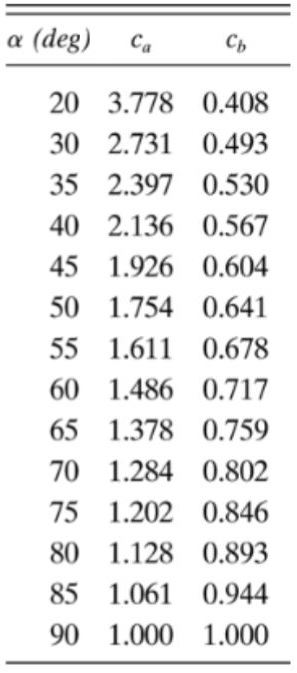
\includegraphics[height=0.35\textwidth, angle = 90]{GeneralContactAlpha.jpg}
    \end{figure}
    \item Calculate \(c_a\), \(c_b\)
    \begin{equation*}
        a = c_a\left( \frac{F m}{n}\right)^{1/3} \hspace{30pt} b = c_b \left( \frac{F m}{n}\right)^{1/3}
    \end{equation*}
    \item Calculate pressure \hspace{40pt} \(P_0 = (1.5F)/(\pi ab)\)
\end{enumerate}
\begin{figure}[h!]
    \hspace{10pt}
    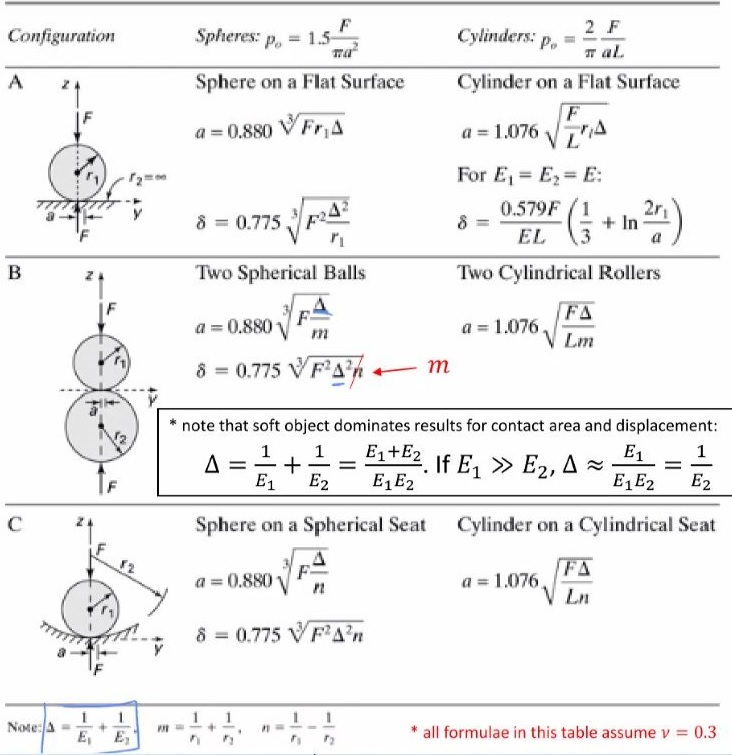
\includegraphics[width=0.4\textwidth]{ContactSimplificationsNUis.3.jpg}
\end{figure}
\subsubsection*{Asymmetric Bending}
Eq. in this section follow directional convention of diagram
\begin{figure}[h!]
    \centering
    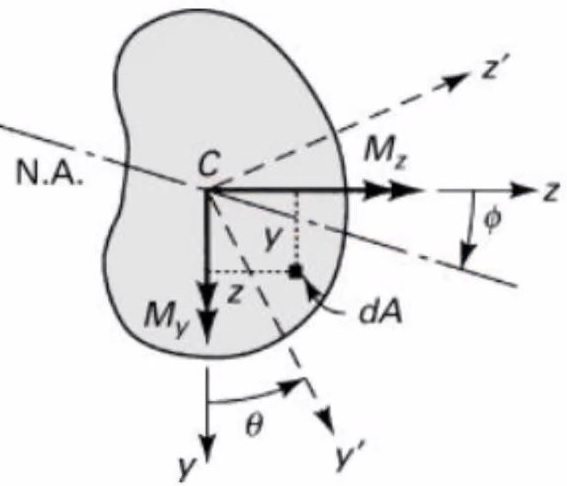
\includegraphics[width=0.25\textwidth]{AsymetricPotato.jpg}
\end{figure}
Solve for \(\sigma_x\) at the point in max compression or tension
\begin{equation*}
    \sigma_x = \frac{(M_yI_y + M_ZI_{yz})z - (M_yI_{yz} + M_zI_y)y}{ I_yI_z - I_{yz}^2}  
\end{equation*}
\begin{equation*}
    tan(\phi) = \frac{y_c}{z_c} = \frac{M_yI_z + M_zI_{yz}}{ M_yI_{yz} + M_zI_y} = \frac{y_c'}{z_c'} = \frac{M_y'I_z'}{ M_z'I_y'}
\end{equation*}
Finding the right coordinate system allows for no transverse deformation, no products of inertia, only moments of inertia. Things are then symmetric, and the body behaves as expected.
\begin{equation*}
    I_y = \int_A z^2dA \hspace{30pt} I_z = \int_A y^2dA \hspace{30pt}  I_{yz} = \int_A yzdA
\end{equation*}
\begin{equation*}
    \text{Where: } \hspace{20pt} dA = idj \hspace{30pt} i,j \in x,y,z \hspace{10pt} i \neq j
\end{equation*}
\underline{Inertias Obey "Mohr's Circle"}\\
\begin{equation*}
    I_{1,2} = \frac{I_y+I_z}{2} \pm \sqrt{\left( \frac{I_y - I_z}{2}\right)^2 + I_{yz}^2} = I_{max},I_{min}
\end{equation*}
\begin{equation*}
    I_y' = \frac{I_y + I_z}{2} + \frac{I_y-I_z}{2} cos(2\theta) - I_{yz} sin(2\theta)
\end{equation*}
\begin{equation*}
    tan(2\theta_p) = \frac{-2I_{yz}}{I_y-I_z}
\end{equation*}


\subsubsection*{Shear Stress}
\begin{equation*}
    \tau = \frac{VQ}{It} \hspace{30pt} q = \frac{VQ}{I} = \tau t \hspace{30pt} t = \text{length of cut}
\end{equation*}
\begin{equation*}
    Q = (\text{Area beyond})(\text{dist from NA to centroid})
\end{equation*}
\begin{equation*}
    I=\sum_{i=1}^N(I_i+A_id_i^2) \hspace{30pt} d_i=d_{cm}-d_{NA}
\end{equation*}


\underline{Shear Center}\\
Balance internal stress and external loading to generate bending only, no torsion.
\begin{figure}[h!]
    \centering
    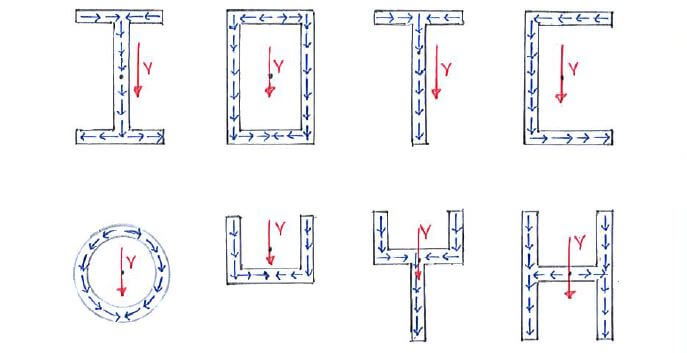
\includegraphics[width=0.35\textwidth]{ShearFlowInBeams.jpg}
\end{figure}
\begin{enumerate}
    \item Resolve shear flow into stress forces along beam cross-section \\
        \begin{equation*}
            F_{a \to b} = \int \int \tau dA \underbrace{=}_\text{const. t} \int \tau tds = \int_0^bqds
        \end{equation*}
    \item Draw a loading with external shear force only, acting at a point on all symmetry axes, with \(e\) dimension labelled
    \item Equate parts 1 and 2, solve for \(e\) 
\end{enumerate}

\subsubsection*{Torsion}
\begin{equation*}
    \rho d\phi = \gamma dx \Longrightarrow \gamma = \frac{\rho \phi}{L} \hspace{30pt} \phi_{\text{circ}} = \frac{TL}{GJ} \hspace{30pt} \tau_{\text{circ}} = \frac{T\rho}{J}
\end{equation*}
No warping of cross-sections, only in and out of plane:
\begin{equation*}
    u = -y \theta_z \hspace{30pt} v = x\theta_z \hspace{30pt} w = w(x,y) \hspace{30pt} \theta = \frac{\phi}{L}
\end{equation*}
\underline{Strains}\\
\begin{equation*}
    \varepsilon_x = \gamma_{xy} = \varepsilon_y = \varepsilon_z = 0 \hspace{20pt} \gamma_{zx} =  \frac{\partial{w}}{\partial{x}} - y\theta \hspace{20pt} \gamma_{zy} =  \frac{\partial{w}}{\partial{y}} + x\theta
\end{equation*}
\underline{Stresses}\\
\begin{equation*}
    \tau_{yz} = G \left(  \frac{\partial{w}}{\partial{y}} +x\theta \right) \hspace{30pt} \tau_{zx} = G \left(  \frac{\partial{w}}{\partial{x}} -y\theta \right)
\end{equation*}
\begin{equation*}
    \sigma_x = \sigma_y = \sigma_z =\tau_{xy} = 0 
\end{equation*}
\underline{Prandtl's Stress Function}\\
\begin{equation*}
    \text{Define }\Phi = \Phi (x,y) \longrightarrow \tau_{xz} =  \frac{\partial{\Phi}}{\partial{y}} \hspace{30pt} \tau_{yz} = - \frac{\partial{\Phi}}{\partial{x}}
\end{equation*}
to satisfy and boundary conditions, and
\begin{equation*}
    \frac{\partial^2 \Phi}{\partial{x^2}} +  \frac{\partial^2 \Phi}{\partial{y^2}} = H = - 2G\theta
\end{equation*}
\begin{equation*}
    \text{Ellipse solution: } \hspace{15pt} \tau_{max} = \frac{2T}{\pi ab^2} \hspace{30pt} \theta = \frac{(a^2+b^2)T}{\pi a^3b^3G}
\end{equation*}
\begin{itemize}
    \item Outer corners of shapes have zero shear stress
    \item Max shear stresses at free surface closest to centroid
    \item Circular cross-section best at holding loads
\end{itemize}
\underline{Membrane Analogy}\\
\begin{itemize}
    \item \(S\) is surface tension
    \item Stress concentrations not accounted for
\end{itemize}
\begin{table}[h!]
    \footnotesize
    \centering
    \begin{tabular}{cc}
        Membrane Problem & Torsion Problem \\
        \hline
        \(z\) & \(\Phi\) \\
        \(1/S\) & \(G\) \\
        \(P\) & \(2\theta\) \\
        \( -\partial z / \partial x \) , \(\partial z / \partial y \) & \(\tau_{zy}\) , \(\tau_{zx}\) \\
        \(2 V\) & \(T\) \\
        \hline
    \end{tabular}
\end{table}
\begin{equation*}
    \underbrace{ \text{rect/unravelled open section}}_\text{Thin-wall} \hspace{15pt} \tau_{max}  = \frac{3T}{bt^2} \hspace{20pt} \theta = \frac{3T}{bt^3G}
\end{equation*}
\begin{equation*}
    \underbrace{ \text{closed section}}_\text{Thin-wall} \hspace{30pt} \tau =\frac{T}{2A_mt} \hspace{30pt} \theta = \frac{1}{2A_mG} \oint \tau ds
\end{equation*}



\subsubsection*{Thick-Walled Pressure Vessels}
\begin{equation*}
    \text{thick-walled if } \hspace{20pt} \frac{r_i}{t} <10
\end{equation*}
\begin{equation*}
    \sigma_r = \frac{a^2P_i - b^2P_o}{ b^2-a^2} - \frac{(P_i - P_o)a^2b^2}{ (b^2-a^2)r^2}
\end{equation*}
\begin{equation*}
    \sigma_\theta = \frac{a^2P_i - b^2P_o}{ b^2-a^2} + \frac{(P_i - P_o)a^2b^2}{ (b^2-a^2)r^2}
\end{equation*}
\begin{equation*}
    \text{if open: } \sigma_z=0 \hspace{30pt} \text{if closed: } \sigma_z = \frac{P_ia^2 - P_ob^2}{b^2-a^2}
\end{equation*}
\begin{equation*}
    \text{if open: } \delta = u = \frac{1-\nu}{E} \frac{(a^2P_i- b^2P_o)r}{b^2-a^2} + \frac{1+\nu}{E} \frac{(P_i-P_o) a^2b^2}{(b^2- a^2)r}
\end{equation*}

Internal P only: \(\sigma_{r,max} , \sigma_{\theta,max}\) at inner\\
External P only: \(\sigma_{r,max}\) at outer, \(\sigma_{\theta,max} \) at inner\\

\underline{Internal and External Pressures}\\
\begin{equation*}
    \text{Let: } \hspace{20pt} R = \frac{b}{a} \hspace{30pt} P = \frac{P_o}{P_i} \hspace{30pt} S = \frac{\sigma_{\theta_i}}{\sigma_{\theta_o}}
\end{equation*}
Then solve for stresses using the following (\(\sigma_{\theta_o} = \sigma_\theta(r=b))\):  
\begin{equation*}
    \sigma_\theta = P_i \frac{1-PR^2}{R^2-1} + P_ib^2 \frac{1- P}{(R^2-1)r^2} \hspace{20pt} S = \frac{1+ \frac{R^2(1-P)}{1-PR^2}} { 1 + \frac{1-P}{1-PR^2}}
\end{equation*}
\underline{Press/Shrink Fits}\\
\begin{equation*}
    \delta = \frac{bP}{E_o} \left( \frac{b^2 + c^2}{c^2 - b^2} + \nu_o \right) + \frac{bP}{E_i} \left( \frac{a^2 +b^2}{b^2-a^2} -\nu_i \right)
\end{equation*}
\begin{equation*}
    P = \underbrace{\text{at surfaces}}_\text{same material}= \frac{E\delta}{b} \left( \frac{(b^2-a^2 ) (c^2-b^2)}{2b^2(c^2-a^2)} \right)
\end{equation*}

\subsection*{Rotating Disks}
\underline{Annular Disk}\\
\begin{align*}
    \sigma_r =& \frac{3+\nu}{8} \left( a^2 + b^2 - r^2 - \frac{a^2b^2}{r^2} \right) \rho \omega^2\\
    \sigma_\theta =& \frac{3+\nu}{8} \left(a^2 + b^2 - \frac{1+3\nu}{3+\nu } r^2 +\frac{a^2b^2}{r^2} \right) \rho \omega^2
\end{align*}
\begin{equation*}
    \sigma_{r,max}(r=\sqrt{ab}) = \frac{3+\nu}{8} (b-a)^2\rho\omega^2
\end{equation*}
\begin{equation*}
    \hspace{-10pt} \delta=u = \frac{(3+\nu) (1-\nu)}{8E} \left(a^2 +b^2 - \frac{1+\nu}{3+\nu}r^2 +\frac{1+\nu}{1-\nu} \frac{a^2b^2}{r^2} \right) \rho\omega^2r
\end{equation*}
\underline{Solid Disk}\\
\begin{equation*}
    \sigma_r = \frac{3+\nu}{8} (b^2 - r^2) \rho\omega^2 \hspace{30pt}  \sigma_{r,max}(r=0) = \frac{3+\nu}{8} b^2\rho\omega^2
\end{equation*}
\begin{equation*}
    \hspace{-10pt} \sigma_\theta = \frac{3+\nu}{8} \left(b^2 - \frac{1+3\nu}{3+\nu} r^2 \right)\rho \omega^2 \hspace{10pt} \sigma_{\theta,max}(r=0) = \frac{3+\nu}{8} b^2\rho\omega^2
\end{equation*}
\begin{equation*}
    \delta= u = \frac{1-\nu}{8E} [(3+\nu)b^2 -(1+\nu) r^2] \rho\omega^2r
\end{equation*}


\subsection*{Strain Energy}
\begin{equation*}
    \hspace{-5pt} U_0 = \frac{1}{2} (\sigma_x\varepsilon_x +\sigma_y\varepsilon_y + \sigma_z\varepsilon_z + \tau_{xy}\gamma_{xy} + \tau_{yz}\gamma_{yz} + \tau_{xz}\gamma_{xz}) = \frac{1}{2}(\sigma : \varepsilon)
\end{equation*}
\begin{align*}
    U_0 =& \frac{1}{2E}(\sigma_x^2 + \sigma_y^2 + \sigma_z^2) -\frac{\nu}{E}(\sigma_x\sigma_y + \sigma_y\sigma_z +\sigma_x\sigma_z) \\
    &+\frac{1}{2G} (\tau_{xy}^2 + \tau_{yz}^2 + \tau_{xz}^2)
\end{align*}
\begin{equation*}
    U = \int \frac{N^2}{2AE}dx + \int \frac{M^2}{2EI}dx + \int \frac{\alpha V^2}{2AG}dx + \int \frac{T^2}{2JG}dx
\end{equation*}
\underline{Castigliano's Theorem}\\
Can be applied with dummy loads \((P=0)\) at locations of interest, or applied to find reaction forces/couples in in-determinant structures.
\begin{align*}
    \delta_i =& \frac{1}{AE} \int N  \frac{\partial{N}}{\partial{P_i}}dx + \frac{1}{EI} \int M  \frac{\partial{M}}{\partial{P_i}}dx \\
    &+\frac{1}{AG} \int \alpha V  \frac{\partial{V}}{\partial{P_i}} dx + \frac{1}{JG} \int T  \frac{\partial{T}}{\partial{P_i}}dx
\end{align*}
\begin{align*}
    \theta_i =& \frac{1}{AE} \int N \frac{\partial{N}}{\partial{C_i}}dx + \frac{1}{EI} ]\int M \frac{\partial{M}}{\partial{C_i}} dx \\
    &+\frac{1}{AG} \int \alpha V  \frac{\partial{V}}{\partial{C_i}}dx + \frac{1}{JG} \int T  \frac{\partial{T}}{\partial{C_i}}dx
\end{align*}
\begin{table}[h!]
    \centering
    \footnotesize
    \begin{tabular}{l|c}
        \(\alpha\) & Value \\
        \hline
        Rectangular & \(6/5\)\\
        I-Beam\(^*\) & \(A/A_{web}\)\\
        Circle &10/9\\
        Thin-wall cyl. & 2
    \end{tabular}
\end{table}
\(^*\) Applies to box beams, and channels too


\subsection*{Buckling}
\begin{equation*}
    P_{crit} = \frac{\pi^2EI}{L_e^2} \hspace{30pt} r= \sqrt{\frac{I}{A}} \hspace{30pt} \frac{L}{r} = \text{slenderness ratio}
\end{equation*}
\begin{table}[h!]
    \centering
    \footnotesize
    \begin{tabular}{l|c}
        Condition & \(L_e\) \\
        \hline
        Pinned-pinned & \(L\)\\
        Fixed-free & \(2L\)\\
        Fixed-fixed & \(L/2\)\\
        Pinned-fixed & \(0.7L\)
    \end{tabular}
\end{table}

\subsection*{Plasticity}
\begin{equation*}
    \sigma_0 = K\varepsilon^n_0 \hspace{10pt} \log(\sigma_0) = \log(K) + n\log(\varepsilon) \hspace{10pt}  \text{zero indicates true}
\end{equation*}
\subsubsection*{Bending Elastic-Perfectly Plastic}
\begin{equation*}
    M = \frac{3}{2} M_{yp} \left(1 -\frac{1}{3}\left(\frac{e}{h} \right)^2 \right) \hspace{30pt} \begin{matrix} 
        e =\text{non-plastic region} \\
        \text{rect. } b\times2h \text{ beams only}
    \end{matrix}
\end{equation*}
\begin{equation*}
    M = \frac{3}{2} M_{yp} \left(1 - \frac{1}{3}\left(\frac{r}{r_{yp}} \right)^2 \right) = M_u \left( 1 - \frac{1}{3} \left(\frac{r}{r_{yp}} \right)^2\right)
\end{equation*}

\subsubsection*{Torsion Elastic-Perfectly Plastic}
\begin{equation*}
    T = \frac{\pi c^3}{6} \left(4 - \frac{\rho_0^3}{c^3} \right) \tau_{yp} = \frac{4}{3}\tau_{yp} \left(1 - \frac{1}{4} \frac{\rho_0^3}{c^3} \right) \hspace{25pt} \phi_{yp} =\frac{\tau_{yp}L}{Gc}
\end{equation*}
\begin{equation*}
    \text{at onset of yield } \hspace{30pt} \frac{\rho_0}{c} = \frac{\phi_{yp}}{\phi} \hspace{18pt} T = \frac{4}{3} \tau_{yp} \left(1 - \frac{1}{4} \frac{\phi_{yp}^3}{\phi^3} \right) 
\end{equation*}







\subsection*{Other}
\begin{equation*}
     \delta=\frac{\textbf{P}L}{EA} \hspace{30pt} \delta_T=\alpha\Delta TL
\end{equation*}



\begin{figure}[h!]
    \centering
    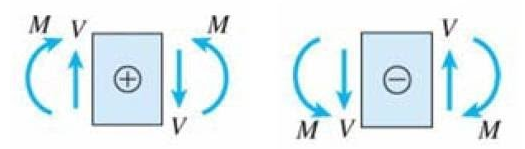
\includegraphics[scale=0.5]{dsc.png}
    \caption*{Deformation sign convention}
    \label{my_label}
\end{figure}

\end{document}